%==================================================================================================
%   LUKES THESIS TEMPLATE 1.2
%   -------------------------
%   This template is based upon the offcial IMM PhD Thesis template, it is enhanced with a number
%   of new features and a number of errors have fixed. This template is intended to be complied to
%   PDF using PDFLATEX and is tested using the MiKTeX 2.9 LaTeX distribution.
%   It is based on the official DTU-IMM Thesis template by Finn Kuno Christensen in 2009.
%   Small bugfixes by Kasper Laursen in 2012 and 2013.
%   -------------------------
%   Last Updated: 2012-09-19
%   Contact: lthhe@imm.dtu.dk
%==================================================================================================
%
%==================================================================================================
% DOCUMENT SETUP
%==================================================================================================
\documentclass[10pt,twoside]{book}                  %Official DTU-IMM Thesis document setup
%
%Set to 'print' for printed version, use 'net' for online version
\def\thesisversion{net}
%
%==================================================================================================
% PACKAGES
%==================================================================================================
\usepackage{LukeThesis}                             %Import Thesis base style
%input{PhDMacros}                                   %Thesis specific macros
%
%==================================================================================================
% THESIS PROPERTIES (Modifiy these fields with your details)
%==================================================================================================
\def\thesisauthor{Constantin Teodor Gherghescu}                     %Author
\def\thesistitle{Inferring Pairwise Co-location from Noisy Bluetooth Signals}               %Title
\def\thesishandin{20-June}                       %Submission date (Day-Month}
\def\thesisdegree{M.Sc.}                              %Degree ('B.Eng', 'B.Sc.', 'M.Sc.' or 'PhD')
\def\thesisyear{2014}                               %Submission year
\def\thesisnumber{????}                             %DTU-IMM Serial number (do not include year)
\def\thesisISSN{0000-0000}                          %ISSN number
\def\thesiskeywords{Keywords are, comma separated}  %PDF keywords
\derivethesisprops                                  %Derive dependent properties
%
%==================================================================================================
% SECTION NUMBERING SETUP
%==================================================================================================
\setcounter{tocdepth}{2}                            %2 adds sections up to subsections
\setcounter{secnumdepth}{3}                         %Subsubsections get a number when this is 3
%
%==================================================================================================
% THESIS STRUCTURE  (Modifiy to include more chapters etc)
%==================================================================================================
\begin{document}
%------------------------
%Pre-frontmatter material
%------------------------
\prefrontmatter
%--------------------
%Frontmatter material
%--------------------
\frontmatter
\pagenumbering{roman}                               %Set frontmatter numbering style
\chapter{Summary (English)}

The goal of the thesis is to provide a method which infers the existence of physical co-location based on Bluetooth RSSI measurements. We gather two types of data through the use of mobile phones, which then we merge in a single set. We use the resulting set to analyse three algorithms: artificial neural networks, logistic regression and Naive Bayes. We vary the parameters of the algorithms and the features used and we compare the results. We look at how well the algorithms can infer co-location, as well as how computationally expensive they are. We finish this paper by recommending the combination of algorithm and feature that had the best results.                                       %English summary of Thesis
\markboth{}{}                                       %Set headings (left)(right)
\chapter{Summary (Danish)}
\begin{otherlanguage}{danish}

Målet for denne afhandling er at ...

\end{otherlanguage}                                   %Danish summary of Thesis
\markboth{}{}                                       %Set headings (left)(right)
\chapter{Preface}

This thesis was prepared at the department of Applied Mathematics and Computer Science at the Technical University of Denmark in fulfilment of the
requirements for acquiring an M.Sc. in Computer Science and Engineering.

%==================================================================================================
% SIGNATURE AREA
%==================================================================================================
\vspace{20mm}
\begin{center}
    \hspace{20mm} Lyngby, \thesishandin-\thesisyear
    \vspace{5mm}
    \newline
  %Update signature image file in line below
    
\includegraphics[scale=0.5]{figures/SignatureDummy}
\end{center}
\begin{flushright}
    \thesisauthor
\end{flushright}
% % % EOF % % %                                     %Preface
\markboth{}{}                                       %Set headings (left)(right)
\chapter{Acknowledgements}

I would like to thank my....

                            %Acknowledgements
\markboth{}{}                                       %Set headings (left)(right)
%------------------
% Table of contents
%------------------
\newpage\mbox{}\newpage
\chaptermark{Contents}
\pdfbookmark{\contentsname}{toc}
\renewcommand{\sectionmark}[1]{\markright{#1}}
\sectionmark{Contents}
\addtolength{\parskip}{-\baselineskip}
\tableofcontents
\addtolength{\parskip}{\baselineskip}
\renewcommand{\sectionmark}[1]{\markright{\thesection\ #1}}
%-------------
% Main content
%-------------
\mainmatter
\chapter{Introduction}

\section{Motivation}

Epidemiology \cite{human_sex}, personal health issues \cite{Madan}, group discovery \cite{5591535}, human mobility \cite{Sun2011929,sevtsuk}, efficient team creation \cite{ECTA, Pentland}, the analysis of academic success \cite{academics}, network theory \cite{networks}, also Fig. \ref{pic:dynamicsf2f}, and psychological research \cite{Rachuri}; all of the above have begun making use of the same notion, one that is difficult to quantify \cite{quant, Wilson}: social connections and social interactions between individuals. And although co-location does not necessarily mean physical social interaction, it is a requirement for it. \cite{Eagle08092009}.

\begin{figure}[h]
	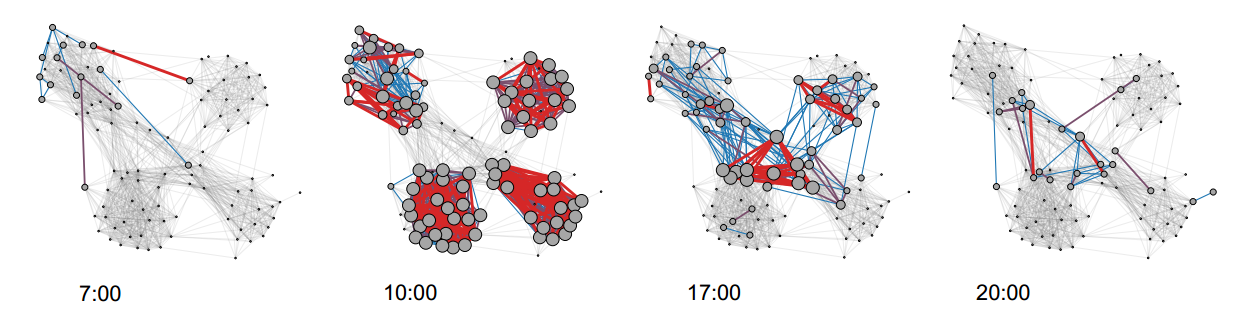
\includegraphics[scale=0.35]{figures/dynamicsf2f.png}
	\caption{Face-to-face interactions over a day for college students. Blue means a low, and red a high frequency of interactions. Image from \protect\cite{Stopczynski}}.
	\label{pic:dynamicsf2f}

\end{figure} 

There are a number of approaches to determining co-location: self-reported data, a more traditional approach, which is prone to cognitive bias, social desirability bias and halo error \cite{Wuchty08092009,gonyea}. A more recent approach involves the use of data provided by modern means of communication, namely mobile phones. This data can come from both the actual phone, in the form of GPS locations or bluetooth readings \cite{Stopczynski}, as well as from the phone company itself in the form of anonymous cell tower records \cite{Onnela01052007, hovel}. This has the advantage of being applicable almost anywhere, because of the high percentage of mobile phone penetration (95.5\% estimated by the International Telecommunication Union in May 2014). 
However, there are approaches that yield better results, but come with financial, environmental or other types of additional cost: RFID tags \cite{catt}, audio-video recordings \cite{audiovideo}, on-body sensors \cite{onbody} and wifi signals \cite{wifi}, just to name a few. 
 
 
\section{Objective}

Given a bluetooth RSSI between two phones, the purpose of this paper is to indicate a method which reliably and accurately determines the existence of pairwise co-location between the people carrying the two phones.

Reliability refers to the fact that multiple tries with the same input, and constant settings ( same machine learning algorithm, same parameters and same training data), will always yield exactly the same result. While accuracy refers to the precision of the algorithm during cross-validation testing, or how close to 100\% it is. 
 
This inference is achieved by applying and analysing multiple machine learning algorithms on a data set consisting of two main parts:
\begin{itemize}
  \item Data automatically recorded by the SensibleDTU data collector app \cite{Stopczynski}
  \item Ground truth data obtained by the test subjects by interacting with the FriendFinder app
\end{itemize}

For each machine learning algorithm the parameter configuration which yields the best results will be chosen, followed by a comparison between the best configurations for each algorithm.      

\section{Scope and limitations}

The paper analyses the data obtained from three test subjects. Each subject has been given the same phone model, Samsung Galaxy Nexus.

While considerable testing has been done with regards to the algorithm parameters, the machine learning algorithms list is by no means exhaustive. There are three main algorithms: Naive Bayes, Neural Networks, and Recursive learning, and an explanation on why a fourth, Hidden Markov Model, is unsuitable for this type of data. 

When analysing data, we only look at the bluetooth RSSI value, and data derived directly while measuring it. For example, given that measurements are taken every five minutes, we at some point look at the length of an uninterrupted string of measurements, or at the measurements taken before and after (if possible) a specific measurement. GPS traces, phone records, infrared sensors, or facebook/email information are not taken into consideration.

\section{Thesis Outline}

The thesis begins with this introduction, which gives an overview of the general theme of the project. The objectives, scope and limitations and thesis outline are all self-defining. 

It continues with a section which describes the data acquisition process and the methodology used to obtain the data from the SensibleDTU database. The section also describes the FriendFinder app, as well as its implementation.

Next, the machine learning algorithms are presented. For each algorithm a theoretical overview is given. The implementation details are discussed, followed by the results obtained by applying it to the data. At the end of this chapter, we do a comparative analysis between the algorithms, followed by the last section, the conclusions, where we will give the final results and recommandations.
                                  %Chapter 1
\chapter{Data acquisition}

The data used in the paper has been gathered over the course of three months, starting in early March and ending in late May. The data has been obtained with the help of three student volunteers. Each volunteer carried a phone, provided by the SensibleDTU project, the same project this thesis is a part of \cite{sensibledtu, Stopczynski}. The phones are Samsung Galaxy Nexus \cite{nexus} and are running the Android operating system \cite{android}. 

Each phone came with two apps. The first recorded regularly a multitude of information, such as Bluetooth RSSI, GPS traces, battery usage and cell tower information, and is a part of the SensibleDTU project \cite{Stopczynski}, while the second allowed the volunteers to manually name the person they are in physical proximity with, and was developed during this thesis. The second app provided the ground-truth information.

This gave rise to two types of data. First, a continuous stream of regular measurements from the first app, and punctual messages from the second app. Below we will go into more detail about how exactly the two types of data look, how are they gathered and finally, how the two are combined to create a unitary set which serves as a basis for the machine learning algorithms.

\section{FriendFinder app}

\subsection{App overview and implementation}

As the app, FriendFinder, is made for the Android operating system, it is implemented using Java for Android \cite{jandroid}. It has a Google App Engine backend \cite{googleapp}. Fig \ref{pic:ff_prtscr} shows the main screen of the app. 

\begin{figure}[h]
	\begin{center}
		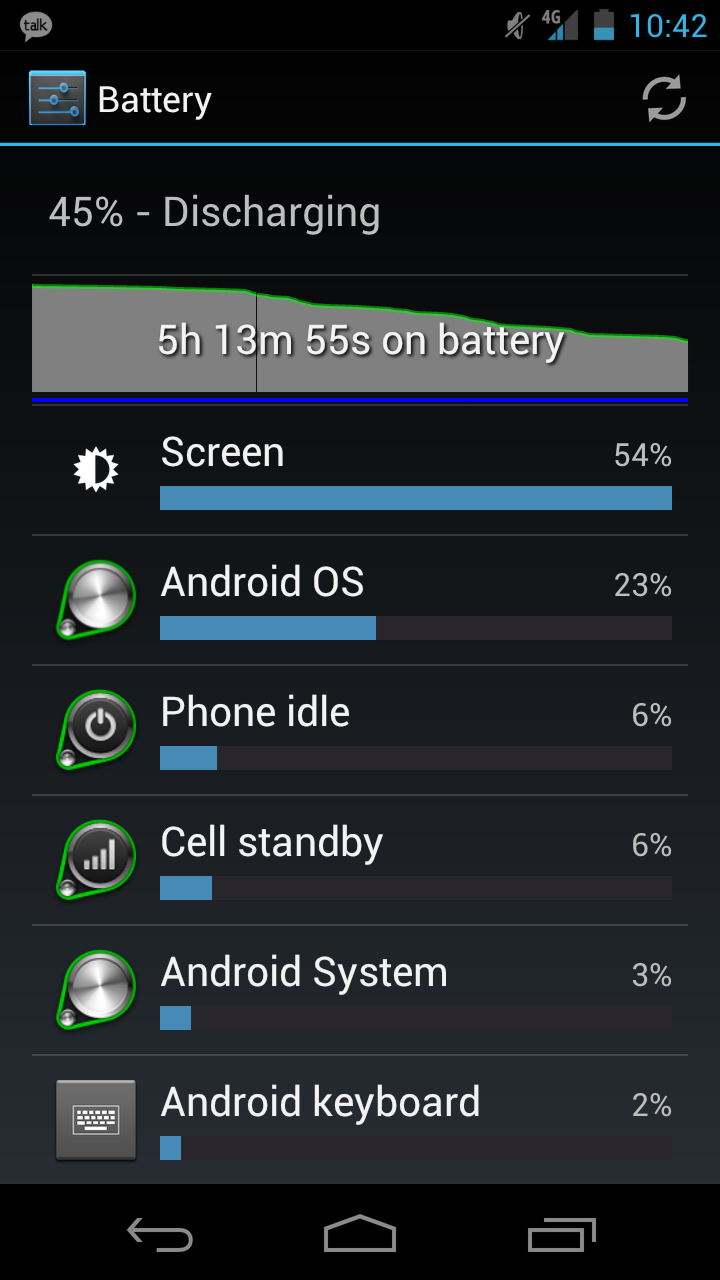
\includegraphics[scale=0.2]{figures/galaxy-nexus-battery.png}
	\end{center}
	
	\caption{FriendFinder app}.
	\label{pic:ff_prtscr}

\end{figure} 

FriendFinder is implemented using a client server architecture, where the clients are the apps installed on the phone, and the server is the Google App Engine. Fig \ref{pic:clientserver} shows an overview of this particular architecture. In this case, the FriendFinder app (in the role of the client) makes a \textit{save data} request to the Google App Engine (the server). The server in turn responds with the result of the operation, either a \textit{succes} or \textit{failure} message.  

\begin{figure}[h]
	\begin{center}
		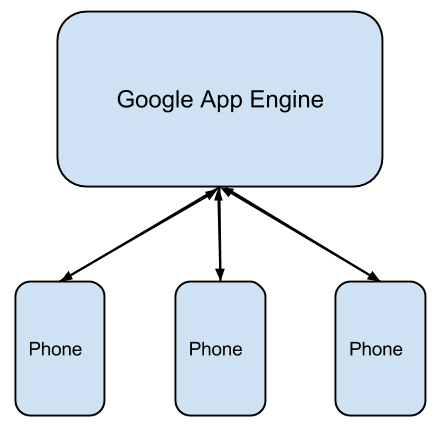
\includegraphics[scale=0.5]{figures/SC_Arch.png}
	\end{center}
	
	\caption{Client Server Architecture used by the FriendFinder app}.
	\label{pic:clientserver}

\end{figure} 

The app contains a single screen (the one showed in Fig \ref{pic:ff_prtscr}), which corresponds to the main activity. Activities are the main building blocks of an Android app, and they are used both to interact with the user, as well as provide additional functionalities \cite{activity}. On the main screen there are buttons for each volunteer. Once one of the volunteers is in physical proximity with another volunteer (as perceived by either one), they both press the button corresponding to each other. A confirmation message is displayed, as can be seen in Fig. \ref{pic:ff_conf}.

\begin{figure}[h]
	\begin{center}
		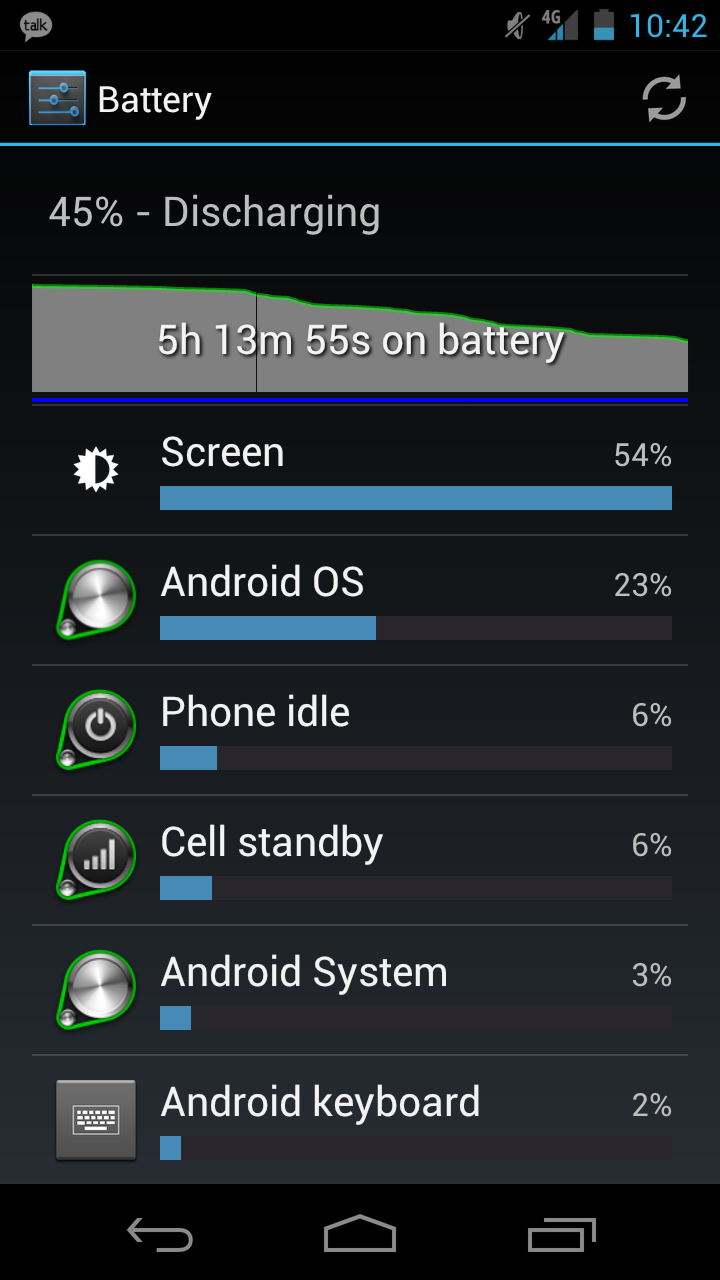
\includegraphics[scale=0.2]{figures/galaxy-nexus-battery.png}
	\end{center}
	
	\caption{Confirmation message on the FriendFinder app}.
	\label{pic:ff_conf}

\end{figure}

For the data to reach the database on the Google App Engine, an internet connection is required. However, the app can also function off-line, by saving all the data locally, and sending it to the on-line database as soon as an internet connection is established. It does this by using an IntentService \cite{intentservice}, which has two main functions:

\begin{itemize}
  \item A first function is to store the data locally, until an internet connection is established.
  \item the second, and most important, is to check periodically for an internet connections. Once an internet connection has been established, all the data is sent to the Google App Engine. The app checks every one minute for internet access. This allows for a relatively fast updating of the database, while at the same time keeping the resource use at a level that does not impede the normal functioning of the phone.
\end{itemize}

The data is stored locally in RAM of the phone (the volatile memory). This is made possible by the relatively small size of the data being saved ( the names of the two people involved, and an ID object that also serves as a timestamp) and the memory capacity of the phone ( approximately 700 MB of RAM). However, this has the disadvantage of being vulnerable to the phone turning off due to lack of battery. The volunteers have been made aware of this fact. 

Once the internet connection is established, the actual sending of the data is a simple matter, done with the help of the Google App Engine API. One thing to mention here is that each data entry is sent individually. If at any point, a \textit{save data} request is met by a \textit{failure} answer, the request is repeated until the \textit{success} message is received. In case of \textit{failure}, subsequent attempts have a one second delay between them. This is done to ensure that the app does not impede the overall functionality of the phone.



\subsection{Data}

Once a button with the name of a person is pressed, the data that is saved on the phone, and eventually sent and saved on the online database has the following format:

\begin{verbatim}
{ID, owner, target}
\end{verbatim}

\begin{description}
  \item[ID] It has a double role. First, the ID is a unique identifier, used for differentiating between multiple entries, as well as for various database operations. This field is required by the Google App Engine. Secondly, the ID also plays the role of the timestamp, used in future computations. While there are valid concerns that the ID might not be unique, due to two people pressing the button at the same time, the fact that the timestamp also includes the millisecond, and the fact that there are only three participants in the project results in an extremely low probability of identical timestamps. Obviously, the timestamp corresponds to the moment the button was pressed, and not the moment the data was sent to the database.  
  \item[owner] This field refers to the owner of the phone, which indicates the person that has made the observation.
  \item[target] This field names the person that has been observed by the owner.
\end{description}

Fig. \ref{pic:dataviewer} shows an example of how the data looks, with the caveat that the \textit{friend} field in the image corresponds to the \textit{target} field in the description above. The saved data was accessed and retrieved by API calls to the Google App Engine.  

\begin{figure}[h]
	\begin{center}
		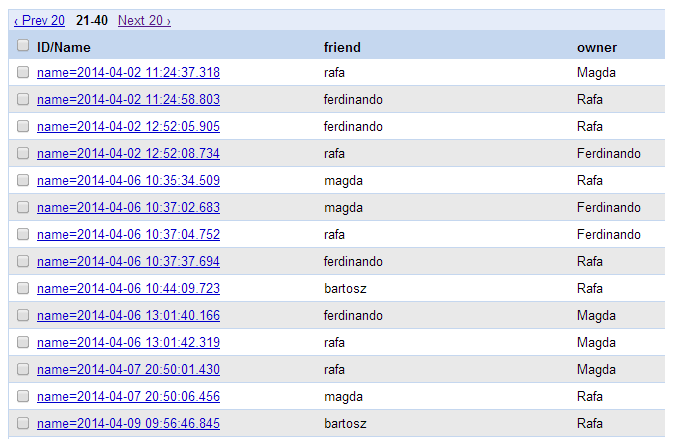
\includegraphics[scale=0.8]{figures/datastore.png}
	\end{center}
	
	\caption{Saved entries for the FriendFinder app}.
	\label{pic:dataviewer}

\end{figure}


\section{SensibleDTU data}

 The second type of data comes from the SensibleDTU data collector app. Based on \cite{Stopczynski,sensibledtu}, we will give a short description of the project, with an emphasis on data collection. We will then focus on the actual data, its form, and how it was collected. 

\subsection{Project overview}
 
 SensibleDTU is the implementation of a large scale study aimed at observing the various interchanges that take place between humans from a social and communications point of view. It aims to collect data on a large group of individuals, most of them students at DTU (Danish Technical University). The collected data consists of, among others, social relations and the networks that form as a result, geographical locations, and, of special interest to this thesis, face-to-face interactions. It does this by using a wide variety of sources, such as questionnaires, the wireless internet on campus, and mobile sensing through smartphones that were handed out to participants. A part of the data gathered through this last method is used in this thesis.
 
The smartphone data gathering is done by using a data collection app, based on the Funf framework \cite{funf}. This data is saved locally on the phone, and it is sent to a secure database server when the app detects the presence of an internet connection. Due to its sensitive nature, great care has been taken to ensure the privacy, security and anonymity of the saved data. Having said that, the three volunteers that participated in the data gathering for this thesis have agreed to the de-anonymization of their Bluetooth information, as it was required in order to merge the two sets of data gathered. 
 
 
\subsection{Data} 

The Bluetooth data is obtained periodically by the data collection app using the Bluetooth probe. Each phone performs a Bluetooth scan every five minutes. The scan lasts 30 seconds. While the 30 second scan lasts, the app saves all Bluetooth devices (that are discoverable) in its proximity, the time at which the scan has been made, as well as the RSSI \cite{vedran}. The data is stored on the phone from where it eventually reaches the secure database server, from where it can be downloaded. 

In order for the data to be used, it first needs to be \textit{cleaned}, as it contains additional meta-data ( fields used by the database for internal accounting), and devices that are not relevant to the thesis. The end result has the following format:

\begin{verbatim}
{time, owner, target,signal_strength}
\end{verbatim}
 
 The above tuple has almost the same format as the one resulted from the FriendFinder app, with the addition of the new field, signal strength. At a first glance, one might think that the two sets of data can be easily combined. However, due to differences in the time when data gathering takes place, de-synchronization and the human factor, obtaining a single data set from the two is not a trivial matter. The following section goes into more detail regarding this issue.
 
\section{Data merger}                                  %Chapter 2
\chapter{Methods for inferring pairwise co-location}

With the data extracted and formatted in suitable manner, as described in the previous chapter, we move on to the main part of the thesis. Given a set of consecutive Bluetooth RSSI measurements, \textit{can we infer co-location?}; and if yes, what is the best way of doing it? 

One way of answering these questions is to simply set a threshold, and split the dataset into two parts: the ones that are above the threshold indicate co-location, while the others do not. That is exactly what \textit{Sekara and Lehmann} did in \cite{vedran}, with convincing results. They set the threshold to \textit{ -80 dBm}. 

On a similar note, we average our two types of data, the ones tagged \textit{yes} and \textit{no}, and we obtain an average of \textit{-64 dBm} for the ones tagged \textit{yes} and an average of \textit{-82 dBm} for the ones tagged \textit{no}. From this result, one can easily see the similarity between the threshold in \textit{Sekara and Lehmann}'s work and the values obtained through this thesis's data. 

The above method can successfully be used under any type of measurement that outputs the RSSI. However, it does not take advantage of the additional information that our method of data gathering has provided, such as temporal information, or the significance of continuous measurements. Below we propose three methods of inferring pairwise co-location in the form of three machine learning algorithms. For each one we will provide a theoretical overview and implementation details, followed by a discussion of the results. The chapter will end with a comparison between the three algorithms where results and computational performance will be taken into consideration.

In Section~\ref{sec:data_merger} we split our data into time windows. At any one point during the execution of the algorithms, we will be referring to a single time window, $w$, for which we want to infer co-location. Of course, additional parameters and features will be used, but even if not specified, every run of any algorithm described below will include as a feature at least the RSSI of $w$.
 
While the parameters and the inputs used differ from one algorithm to another, one thing that remains constant across all of them is the testing methodology, described in the following section.

\section{Testing methodology}

In order to test the accuracy of the algorithms, we use cross-validation, a well recognized method for computing accuracy estimations \cite{kohavi1995study}. The technique is used here for obtaining an accuracy score for each algorithm and its variations, so that a comparison can be made at the end. Broadly speaking, cross-validation refers to the techniques used to partition the main dataset into two sets: a \textit{training} set, used in the initial phase for training the algorithms, and a \textit{testing} set, used for validating the algorithm with \textit{unseen before} data, after the training has finished. Two methods were used: k-fold validation, with $k = 10$ \cite{kohavi1995study}, and repeated random sub-sampling validation, with a $80-20$ proportion \cite{segaran}. 

\begin{itemize}
  \item K-fold validation is done by partitioning the data in k sets. One set is used for testing, while the the other $k-1$ are used for training. The processed is repeated $k$ times, once for each partition. The end result is the average over all $k$ results obtained. 
  \item For random sub-sampling validation, the dataset is partitioned into two sets. The entries are randomly assigned to one of the sets based on the proportion established at the beginning. For this type of validation, the test has been repeated 100 times, and the results averaged.   
\end{itemize}

During the execution of the tests, both k-fold validation and repeated random sub-sampling validation output extremely similar results. For this reason, when presenting an algorithm score, that score will be the average of the two methods. 


\section{Neural Networks}

A first approach aims to use artificial neural networks (ANN) in order to infer co-location. Specifically, this section will deal with feed-forward ANNs, both from a theoretical and a practical point of view. 

\subsection{Theoretical overview}

The introduction of backpropagation by Rumelhart et al. \cite{rumelhart} paved the way for the development of the modern artificial neural network. In their current form, ANNs can be described as a set of processing units, called \textit{neurons}, or \textit{artificial neurons} that communicate between each other. 

The general layout of a feed-forward ANN can be seen in Fig. \ref{pic:ann}. It consists of an input layer, one or more hidden layers and an output layer. The number of \textit{neurons} on the input layer is equal with the number of features that represent the object we need to classify. The number of \textit{neurons} in the output layer usually equals the number of classes the objects need to be classified in. The number of hidden layers, and the number of \textit{neurons} in those layers varies greatly from problem to problem, and will be discussed in the next section, which tackles the implementation details.
In addition to the processing units, the other major components of a feed-forward network are the links between the \textit{neurons}. They type of ANN described here is feed-forward, which means the links are uni-directional. Information only moves from the input \textit{neurons}, to the \textit{neurons} in the hidden layers, to the \textit{neurons} in the output layers. For example, in Fig. \ref{pic:ann}, information only moves from left to right \cite{annintroduction2}.  

\begin{figure}[h]
	\begin{center}
		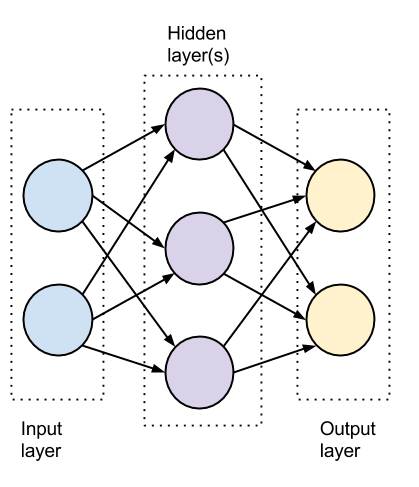
\includegraphics[scale=0.6]{figures/ANN.png}
	\end{center}
	
	\caption{General structure of an ANN.}
	\label{pic:ann}

\end{figure} 

An artificial neural network gets its name from the similarity it has with the biological network of neurons one finds in the human or animal brain. The same can be said about the way it works. Each \textit{artificial neuron} receives an input from all the other \textit{neurons} on the previous layer (or they receive outside input if they are on the input layer). Once all the inputs are received, the \textit{neuron} in question processes them and outputs the result to \textit{neurons} on the next layer \cite{annintroduction}. Fig. \ref{pic:neuron} shows the details of an \textit{artificial neuron}.

\begin{figure}[h]
	\begin{center}
		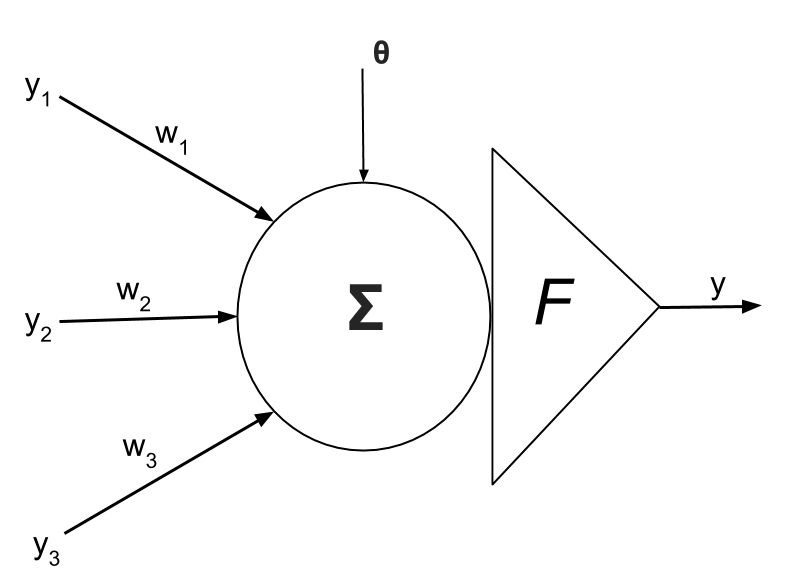
\includegraphics[scale=0.3]{figures/neuron.png}
	\end{center}
	
	\caption{Structure of an artificial neuron.}
	\label{pic:neuron}

\end{figure}

Each link between \textit{neurons} is characterized by a weight, $w_i$. A \textit{neuron} applies a so-called \textit{activation function} on the weighted sum of the inputs, and outputs the result. Sometimes, a bias is used: $\theta$. Thus, the output of single \textit{neuron} can be expressed as:

\begin{equation*}
y = F(\sum_i w_i y_i + \theta)
\end{equation*}

\begin{description}
  \item[$y$]   The output of the current \textit{neuron}.
  \item[$F$]   The activation function. This is usually either the \textit{sigmoid} function, $y = F(x) = \frac{1}{1 + e^{-x}}$, or the \textit{tanh} function \cite{annintroduction}.
  \item[$w_i$] The weight of an input link.
  \item[$y_i$] The input, either from a previous layer of \textit{neurons}, or a from outside the network.
  \item[$\theta$] Bias
\end{description}

In order for the network to output the expected result when presented with an input, it has to be set up. That translates into assigning appropriate values to the weights corresponding to the links between \textit{neurons}. One way of doing this is to manually assign the values. However, this implies a priori knowledge, which is not possible in most cases. The other choice is to \textit{train} the network. 

The training method used here is backpropagation, first introduced in \cite{rumelhart}. The intuition behind is as follows. We randomly assign values to the weights $w_i$ in the ANN. We apply an input to the network, whose result we already know, and compare the outputted result with the correct one. The aim is to minimize the difference. 

While the mathematical procedure through which researchers have reached backpropagation is outside the scope of this thesis, based on \cite{annintroduction} we will present the general equations used in the implementation of the algorithm:

We modify each weight with:  
\begin{equation*}
\Delta w_k = \alpha \delta_k y_k
\end{equation*}

Where $\alpha$ is the learning rate, $y_k$ is the input value on link $k$, and $\delta_k$ is computed as follows:
\begin{equation*}
\delta_k = F'( \sum_i w_i y_i + \theta ) \sum \delta_l w_{kl}
\end{equation*}

Where $\delta_l$ is used in the next layer, and $w_{kl}$ represents a weight between the current layer and the next one. This process continues recursively, until we reach the output layer. In order to finish the computations, we need the $\delta_o$ which corresponds to the output layer:  

\begin{equation*}
\delta_o = (d - y) F'(\sum_i w_i y_i + \theta)
\end{equation*}

Where $d$ represents the expected output, and $y$ the desired output. As one can easily see, we begin from the output layer with computing $\delta_o$, and updating the corresponding weights. We then move further one layer, and compute the corresponding $\delta$ values. We continue to go back until we reach the links that connect to the input layer. From this procedure the \textit{back} in \textit{backpropagation} comes from. 

\subsection{Results}

For implementation purposes we used a Python neural network, available at \cite{issam}. The network used has, besides the mandatory input and output layers, a single hidden layer (which is enough \cite{Hornik1989359,Hartman,cybenko}). 

The number of \textit{neurons} in the hidden layer differs greatly from problem to problem, with some authors suggesting any number between the number of \textit{neurons} in the input layer, to up to two times that value \cite{Stathakis}. Due to the relatively small number of features extracted from the phone data, we have run tests varying numbers of hidden units in the above mentioned range. 

During the testing, different values for the $\alpha$ parameter have been tried, in the end, the values that yielded the best results being between 0.15 and 0.4, with little variation. As such, all the tests that are done below are done with an $\alpha$ parameter of 0.2. 

We begin our testing with the most basic case. We use a single feature, the measured Bluetooth RSSI. The plot in Fig.~\ref{pic:ann_single} details the results obtained. While the accuracy is acceptable, we can easily see that varying the number of hidden nodes in the hidden layer has no impact on the result. 

\begin{figure}[h]
	\begin{center}
		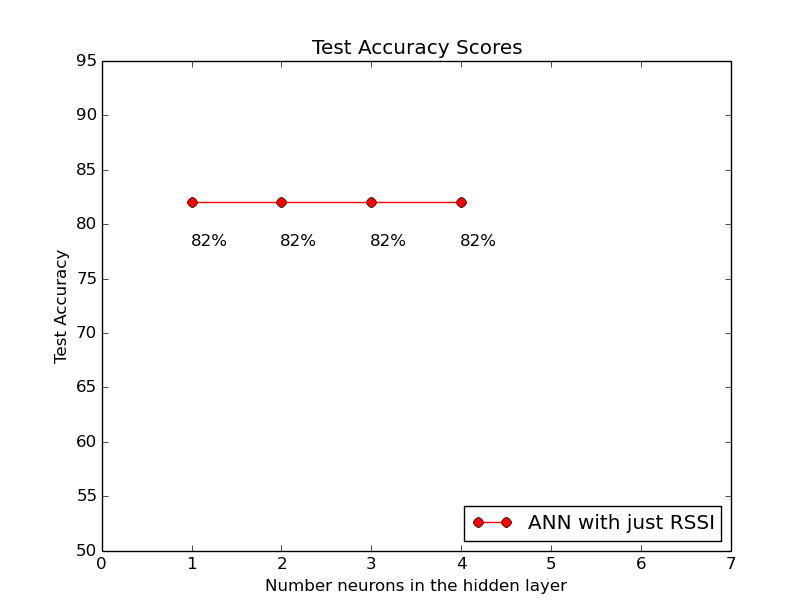
\includegraphics[scale=0.6]{figures/ann_simple.png}
	\end{center}
	
	\caption{Test accuracy for ANN when just the RSSI is used as a feature. The standard deviation is approximately $\sigma = 0.4$, regardless of the number of neurons used.}
	\label{pic:ann_single}

\end{figure}

Next we try to make use of the notion of chains, as it was defined in Section~\ref{sec:data_merger}. When trying to infer co-location for a specific time window, we also look at the RSSI of the windows that are in the same chain, but before it. We gradually increased the number of \textit{neurons} in the hidden layer, as well as the number of windows we take into consideration. 

As we increased the number of windows, the length of the chains becomes a problem. Different chains have different lengths, but the number of features in the ANN remains constant. For example, when using four previous windows, and a chain has only a length of three, even in the best case scenario, we still have two missing features. 

One way to deal with this problem is to simply discard the cases that are missing values. However, this introduces significant bias into the data, as observation of the dataset has shown that shorter chains are more likely to belong to the category tagged with \textit{no}. By discarding them, we greatly reduce the number of samples tagged with \textit{no}, thus unbalancing the overall proportion of training and testing data. As such, we used imputation to replace the missing values. Two approaches were used.

A first approach used mean imputation. We replaced the missing data with the average of the values in the chain. Fig.~\ref{pic:ann_params2} shows the results obtained. Secondly, we used last observation carry forward \cite{locf}, as it involved items ordered by time value. The results can be seen in Fig.~\ref{pic:ann_params1}. Consideration has been given to multiple imputation \cite{rubin2009multiple}, however, its cost, and the next result made it unsuitable.  

\begin{figure}[h]
	\begin{center}
		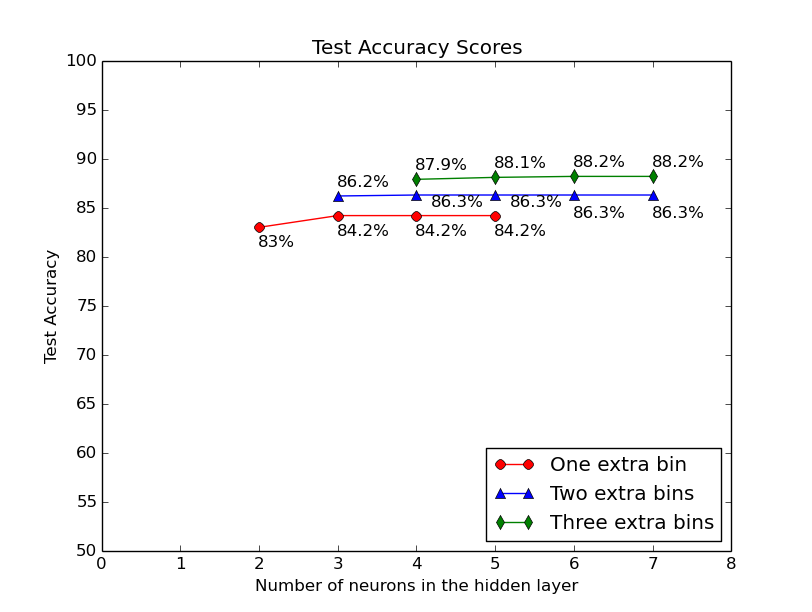
\includegraphics[scale=0.6]{figures/ann_params2.png}
	\end{center}
	
	\caption{Test accuracy for ANN when the RSSI for the current and previous time windows are used as features, with mean imputation. The standard deviations are $\sigma=\lbrace 1.5,1.2,1.2,1.1 \rbrace $ for one extra time window, $\sigma=\lbrace 2.2,2.4,2.4,2.5 \rbrace $ for two and $\sigma=\lbrace 2.7,2.7,2.7,2.7 \rbrace $ for three}
	\label{pic:ann_params1}

\end{figure}

As we increase the number of time windows, for mean imputation, the accuracy increases. However, this is due to the uniformization of data, as every value that is missing is replaced with the average. As the average is almost the same between the testing set and the learning set, we end up with entries who sometimes look extremely alike. When entries are full of averages, the difference is made by the real data. As the number of time windows with real data decreases, this choice of parameters comes closer and closer to the basic one. However, even with one extra bin, this choice of parameters is an improvement over it, as every extra time windows has the chance of providing new data.   

\begin{figure}[h]
	\begin{center}
		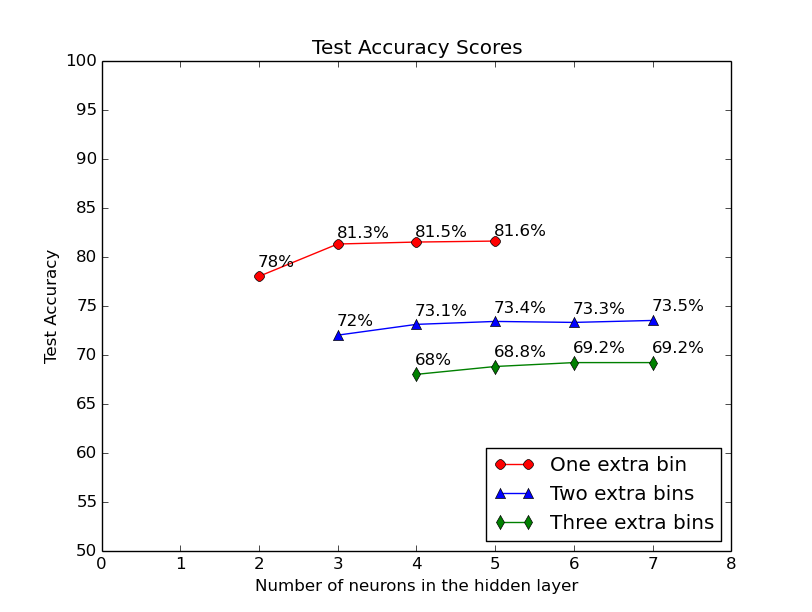
\includegraphics[scale=0.6]{figures/ann_params1.png}
	\end{center}
	
	\caption{Test accuracy for ANN when the RSSI for the current and previous time windows are used as features, with last observation carry forward imputation. The standard deviations are $\sigma=\lbrace 2,2.3,2.4,2.3 \rbrace $ for one extra time window, $\sigma=\lbrace 2.9,3,3,3.2 \rbrace $ for two and $\sigma=\lbrace 4.2,3.9,4.1,4.2 \rbrace $ for three}
	\label{pic:ann_params2}

\end{figure}

Running the algorithm with a last observation carry forward strategy for replacing missing values produces negative results. Even taking into consideration the best result of this set, obtained with only one extra time window, we are still below or close to the score of the basic set.  As we increase the number of time windows used, the accuracy drops markedly, with an almost 7\% jump downwards between one and two extra time windows, and a 4\% drop between two and three extra time windows. This choice of parameters is unsuitable for this algorithm.    

The additional information provided by the chain can improve the result. However, the previous approach had a number of issues, related to missing values, and the choice of how many extra time bins should be taken into consideration. For the next set of parameters, we only use two features: the RSSI of the current window, and the length of the chain the window is a part of. This has the strength of avoiding any bias introduced by imputation, while at the same time making almost full use of the additional information provided by the chain. Fig.~\ref{pic:ann_chain} shows the test accuracy for this choice of features.

\begin{figure}[h]
	\begin{center}
		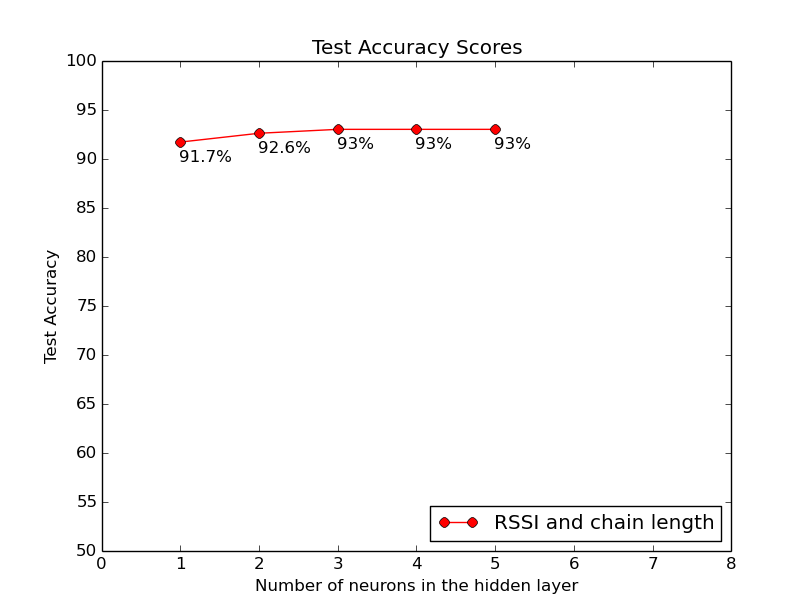
\includegraphics[scale=0.5]{figures/ann_chain.png}
	\end{center}
	
	\caption{Test accuracy for ANN when the RSSI and the chain length are used as features. Standard deviations are $\sigma=\lbrace 0.6,0.7,0.7,0.7 \rbrace $}
	\label{pic:ann_chain}

\end{figure}

Finally, Fig.~\ref{pic:ann_total} shows a plot with a comparison between the best results for each choice of parameters. Clearly, using just the current window RSSI and the chain length is the best choice. While providing just a minor increase in computation cost by adding just one extra new feature, it is better than the basic case by more than 10\%. The parameter set using mean imputation comes close, but still produces inferior results. Furthermore, the use of imputation raises questions regarding the validity of the obtained result, as well as over-fitting. 

Across the entire suite of tests, the variation in the number of \textit{neurons} had little to no impact on the overall accuracy of the tests. Even with a minimum number of \textit{neurons}, the results were extremely close to cases where four or five were used. The extra \textit{neurons}, however, did had an impact on the overall performance. The difference between using three \textit{neurons} instead of one translated into a doubling of the training and running time. 

\begin{figure}[h]
	\begin{center}
		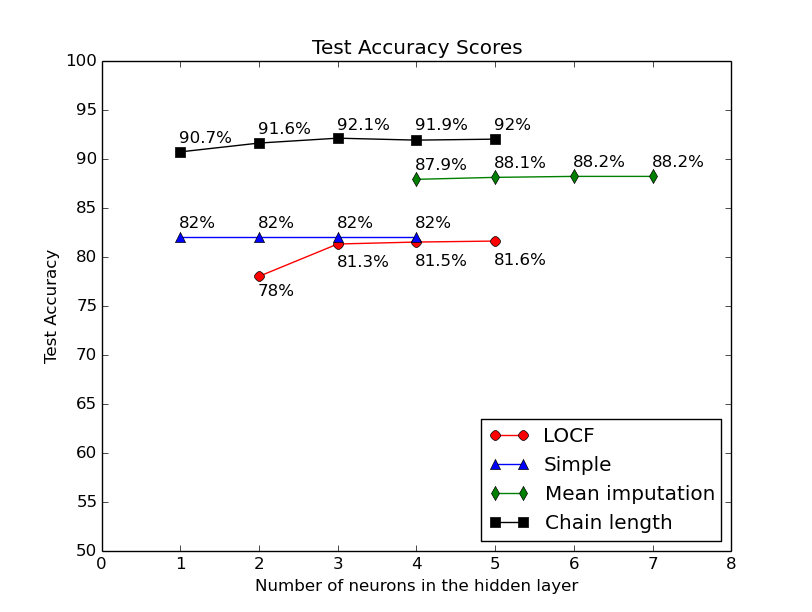
\includegraphics[scale=0.6]{figures/ann_total.png}
	\end{center}
	
	\caption{Comparison between test accuracy for the best cases for each set of parameters.}
	\label{pic:ann_total}

\end{figure}
     

\section{Logistic regression}

In order to meet the objective stated at the beginning of this thesis, we look at the measured Bluetooth RSSI, and some adjacent data, and we try to decide if we have co-location. This can be expressed as the output(response) variable is depending, in some form, on the input(explanatory) variables \cite{logmodel1}. This immediately leads to the idea of regression. The most basic example of this is the linear regression. However, linear regression has an output variable that is continuous, which is unsuitable for the problem raised by this thesis.

Indeed, here we have a dichotomous outcome. Given a set of measurements, there either is or there isn't co-location. For these types of situation, a different type of regression is required, namely logistic regression. 

\subsection{Theoretical overview}

Although usually regressions are used to either predict or estimate a certain value, logistic regression is actually a classifier, thus suitable for our problem. 

The foundation of the logistic regression consists of the logistic function:
\begin{equation*}
f(y) = \frac{1}{1+e^{-y}}
\end{equation*}

Fig.~\ref{pic:logit} shows the plot of the logistic function. It has several attractive qualities. Based on \cite{kleinbaum2010logistic}:

\begin{itemize}
  \item Its output values are between $0$ and $1$. Thus it can easily map probabilities, which is the result of the logistic model.
  \item Looking at Fig.~\ref{pic:logit}, we can discern the presence two points after which the function increases(decreases) significantly , which can be considered activation thresholds, when looking from the point of view of a classifier.  
\end{itemize}

\begin{figure}[h]
	\begin{center}
		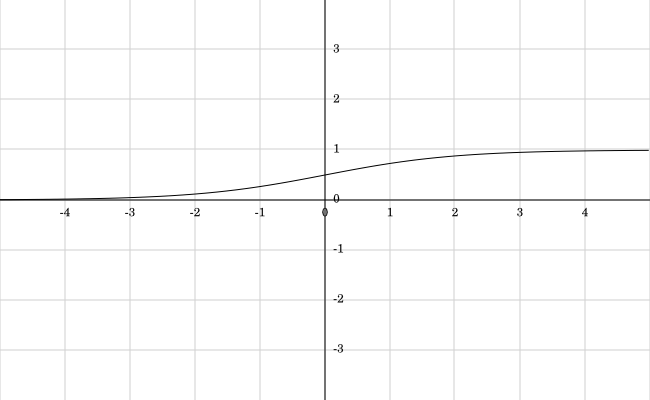
\includegraphics[scale=0.5]{figures/logit.png}
	\end{center}
	
	\caption{Plot of the logisitic function.}
	\label{pic:logit}

\end{figure}

Based on \cite{kleinbaum2010logistic,logmodel1,statistics}: for a set of measurements, the logistic model computes the probability that they belong to either one of the categories. We wish to model the dependence between $X$, which consists of a set of variables $X = \lbrace X_1,X_2,X_3,... \rbrace $, which express the features, and $p(X) = Pr(Y \vert X)$, where $Y$ represents the classifier labels. Using the above logistic function, we can write:
\begin{equation*}
p(X) = \frac{1}{1+e^{-X}}
\end{equation*}

But $X$ can be written as a linear combination of the input variables: $X = \beta_0 + \beta_1X_1 + \beta_2X_2 ... $. Replacing in the above equation we obtain:
\begin{equation*}
p(X) = \frac{1}{1+e^{-(\beta_0 + \beta_1X_1 + \beta_2X_2 ...)}}
\end{equation*}

We also need to compute the \textit{logit}, the inverse of the above function, which looks very much like a regular linear regression:
\begin{equation*}
ln\frac{p(X)}{1 - p(X)} = \beta_0 + \beta_1X_1 + \beta_2X_2 ...
\end{equation*}

All that is left now is to estimate the unknown quantities $\beta_0, \beta_1, \beta_2...$, through the process of training. This is usually done with maximum likelihood estimation \cite{menard2009logistic}. Intuitively, the method looks for estimates of $\beta_0, \beta_1, \beta_2...$, so that the results obtained using those estimates come very close (or as close as they can) to the expected result. The maximum likelihood estimation makes use of the likelihood function:

\begin{equation*}
l(\beta) = \prod_ip(X_i)[1 - p(X_i)]
\end{equation*}
 
Where the first term corresponds to cases that belong to one category, and the second to cases that belong to the other category. The estimations for $\beta_0, \beta_1, \beta_2...$ are chosen so that the above function is maximized. Solving the above equation entails the use of computationally intensive iterative methods \cite{logmodel1}, and is outside the scope of this paper. Once discovered, the estimations are plugged back in the logit, and the model can be used for classification.
 
\subsection{Results}

We used the Scikit-learn \cite{scikit-learn} implementation for the logistic regressor. For testing purposes we used the same sets of parameters as before. The results can be seen in Fig. \ref{pic:logic_tot}.

\begin{figure}[h]
	\begin{center}
		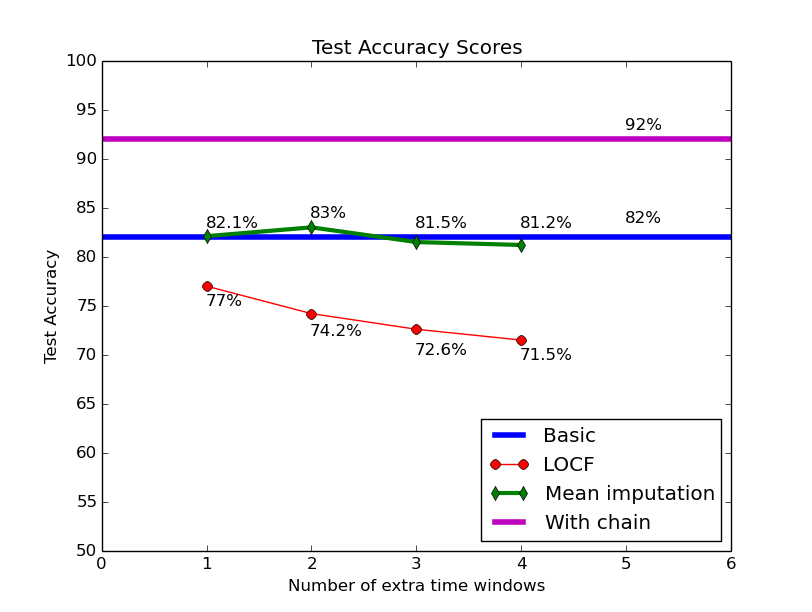
\includegraphics[scale=0.7]{figures/logic_tot.png}
	\end{center}
	
	\caption{Testing results for logistic regression. Standard deviation is $\sigma= 0.3 $ for basic, $\sigma= 0.5 $ for chain, $\sigma=\lbrace 1.4, 1.6, 1.9, 2 \rbrace $ for mean and  $\sigma=\lbrace 3.6, 3.7, 3.7, 4 \rbrace$ for LOCF}
	\label{pic:logic_tot}

\end{figure}

For the basic case, where only the Bluetooth RSSI measurement is used, the accuracy reaches 82\%. We then continue the tests with the use of multiple time windows. Again, in case of missing windows, we use imputation, both mean imputation and last observation carry forward. 

Increasing the number of time windows used has little effect on the mean imputation parameter set, it peaking at 83\%, when two extra time windows were used. This value comes very close to the score obtained with the basic set, and also introduces a high amount of computational overhead, from the algorithm (as we add more features, more values need to be estimated), as well as the database structure(as the chain structures need to be traversed). Overall, this choice of parameters brings little against the basic set.

The same cannot be said by the variation that uses last observation carry forward. Increasing the number of time windows taken into consideration has a significant effect on the overall accuracy of the algorithm. Unfortunately, it is not a positive one. As we increase that number, the accuracy decreases dramatically. Even with one extra time window, the score we obtain is lower than even the basic case. When we move to two extra windows, the score drops to 74.2\%, to 72.6\% for three windows, and 71.5\% for four windows, and the trend continues. Clearly, this choice of parameters is not suitable for this particular algorithm. 

The last choice of parameters is the Bluetooth RSSI of the current time window and the length of the chain it belongs to. This set of parameters provides a significant improvement over all the other cases, with an accuracy of almost 92\%. In addition to the improved test score, this choice requires only one new feature to be added to the algorithm, in comparison to the base case.

Although the results obtained using mean imputation are usable, the fact that they are almost identical to the base case gives us no reason to chose it. Overall, the chain length has the most impact on accuracy, while at the same time avoiding the pitfalls of imputation, making it the best choice for logistic regression. 

\section{Naive Bayes}

Given that the two algorithms discussed above outputted similar results in their best cases, we considered using a more simple algorithm to check if we obtain the same results. Naive Bayes was the choice.

\subsection{Theoretical overview}

Naive Bayes is a probabilistic classifier \cite{forty}. At its core, the Naive Bayes classifier uses Bayes theorem:

\begin{equation*}
p(Y \vert X) = \frac{p(Y)p(X \vert Y)}{p(X)}
\end{equation*}

In case of the classifier, $Y$ is a variable over the classes the data needs to be classified in, where $X$ is a variable representing the features. $X$ can also be replaced by multiple variables expressing the presence of multiple features: $X_1,X_2,X_3,..., X_n $. Based on \cite{forty}, replacing this in the theorem we obtain:

\begin{equation*}
p(Y\vert X_1,X_2,X_3,..., X_n) = \frac{p(Y)p(X_1,X_2,X_3,..., X_n\vert Y)}{p(X_1,X_2,X_3,..., X_n)}
\end{equation*}

One thing to mention here is that when used for classification by comparing values, for the above model, the item located at the denominator is constant (that is, it does not depend on $Y$), and does not need to be computed. 

And here, the \textit{naive} part of the classifier comes in. We assume that the feature variables are independent (the assumption is obviously wrong, however, it has been shown to have good results in practice \cite{rish2001empirical}). Thus we can write:

\begin{equation*}
p(X_1,X_2,X_3,..., X_n\vert Y) = \prod_{i=1}^np(X_i \vert Y)
\end{equation*}

Replacing in the equation above, we obtain:

\begin{equation*}
p(Y\vert X_1,X_2,X_3,..., X_n) = \frac{p(Y)\prod \limits_{i=1}^np(X_i \vert Y)}{p(X_1,X_2,X_3,..., X_n)}
\end{equation*}

This gives us the model. It computes the probabilities that a certain feature vector, representing an object, belongs to either category. While the probabilities calculated are not correct, the relation between them is valid. That is, if an object to be classified has a higher probability of belonging to class $A$ compared to the probability of belonging to class $B$, than that object probably belongs to class $A$. 

The parameters are estimated through training, using maximum likelihood \cite{zhang2004optimality} (which is outside the scope of this paper). However, depending on the type of data we wish to classify, we need to assume a specific feature distribution, usually called \textit{event model} \cite{mccallum1998comparison}. For continuous data, the Gaussian distribution is usually used, while for discrete features Bernoulli and multinomial distributions are used \cite{mccallum1998comparison}.

\subsection{Results}

We used the Scikit-learn \cite{scikit-learn} implementation for the Naive Bayes classifier. Due to the continuous nature of the features, we used the Gaussian distribution. For testing purposes we used the same sets of parameters as before. The results can be seen in Fig. \ref{pic:naive_tot}.

\begin{figure}[h]
	\begin{center}
		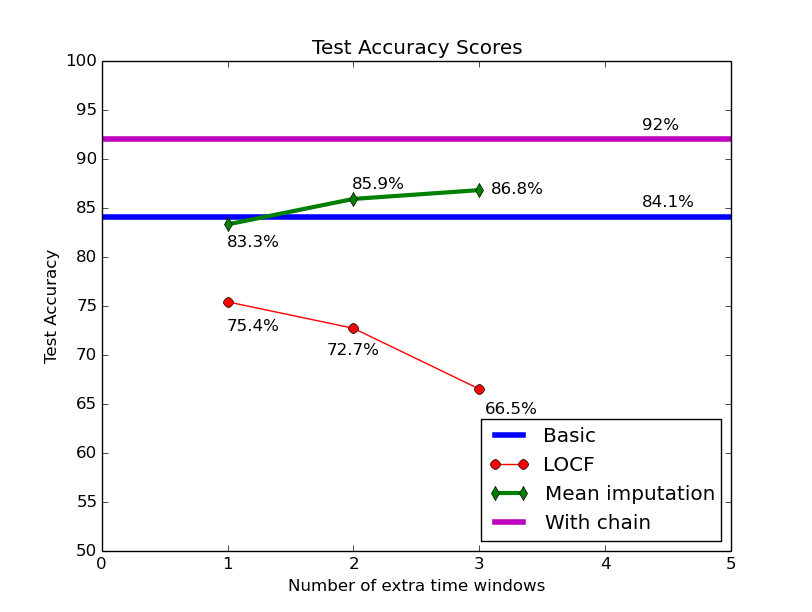
\includegraphics[scale=0.7]{figures/naive_tot.png}
	\end{center}
	
	\caption{Testing results for Naive Bayes. Standard deviation is $\sigma= 0.4 $ for basic, $\sigma= 0.4 $ for chain, $\sigma=\lbrace 1.6, 2, 2.2 \rbrace $ for mean and  $\sigma=\lbrace 3.7, 3.8, 4.4 \rbrace$ for LOCF}
	\label{pic:naive_tot}

\end{figure}

We obtain an accuracy of a bit over 84\% for the basic case, where only the Bluetooth RSSI has been used. We then move to testing with multiple time windows, as it has been described in the sections above.

The variation with last observation carry forward has a terrible result, dropping a staggering 10\% compared to the base case, to a 75.4\%. Increasing the number of time windows used further deteriorates the result, reaching a low of 66.5\%. As we have come to expect, this choice of parameters does not provide a usable result.

Using mean imputation, we obtain a small improvement over the base case, but not right from the start. When only one extra time window is used, the result is slightly worse. By going to two windows we obtain a better 85.9\% score, while further increasing the number of windows does not provide a significant improvement. 

The last set of parameters used, RSSI and chain length provide the best results, with a score of 92\%, a marked improvement over the other choices.  

\section {Algorithms comparison and discussion}

We compare the three algorithms from two perspectives: results and performance.

\subsection{Algorithm score}

Fig. \ref{pic:total_tot} shows an overview of the results obtained using the three algorithms. For each algorithm, and for each major version of parameters used (base, last one carry forward imputation, mean imputation and chain length), the best variation was selected. This includes, for example, the appropriate number of neurons in the hidden layer for ANNs, or the extra number of time windows used. 

For the base case, we obtain similar scores across the board, with a slight advantage for Naive Bayes. This can be explained by the straight-forward manner of the algorithm in comparison with the other two, in combination with the simplicity of the feature set, where only the RSSI was used. The problem simply devolves into a threshold situation, where RSSIs over a certain value have a higher probability of being classified as co-location. Furthermore, the \textit{naive} assumption of the algorithm becomes correct, as we only used one feature.

When using imputation, the results vary between the different sets of parameters and algorithms. However, one thing becomes clear: last observation carry forward always produces subpar results, even when compared to the base case. The only case in which it comes close is ANN, and even then it does not surpass it. 

Mean imputation produces better results, always surpassing the base case for every algorithm. Between the three, ANN produces the best improvement and also holds the highest test score. And if we were to stop our analysis here, ANN using mean imputation would be the most accurate combination.  

\begin{figure}[h]
	\begin{center}
		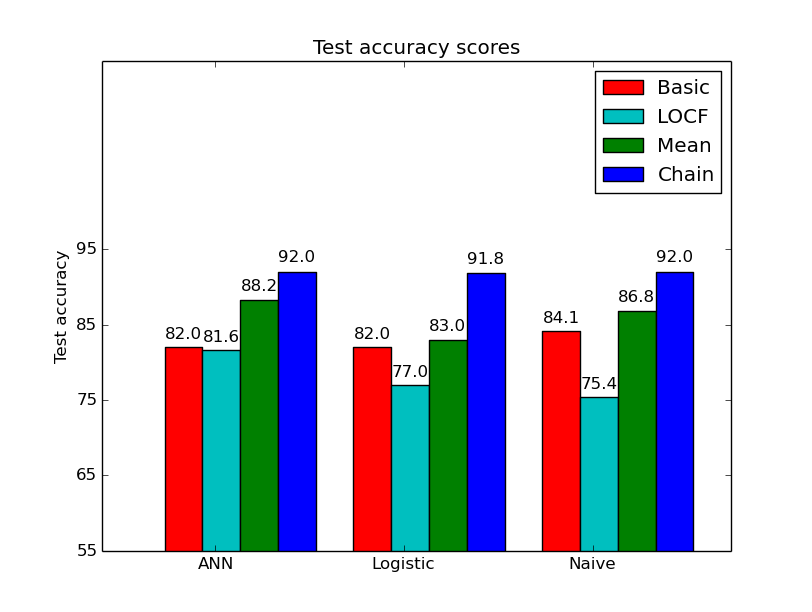
\includegraphics[scale=0.6]{figures/total_tot.png}
	\end{center}
	
	\caption{Summary of results obtained across all three algorithms.}
	\label{pic:total_tot}

\end{figure}

However, that is not the case, as the best results were obtained, every time, by using the length of the chain as a feature, in addition to the RSSI. The obtained test scores are extremely similar for all the algorithms, hovering around the value of 92\%. This brings to light the notion that not only Bluetooth RSSI matters, but also the length of time for which we can maintain a Bluetooth connection, with longer times being indicative of the presence of co-location.  

When taking into consideration just the base case and the best case(chain length), a pattern becomes obvious: the choice of algorithm does not matter. This is proved by the almost identical test scores for all three algorithms. Another influence on the similar scores obtained by the classifiers is the small number of features used. Under these circumstances, the features that are used become extremely important: this is why the results obtained with artificially created data through imputation vary so much.

Using the set of features indicated here, from an accuracy point of view, the choice of algorithm does not matter. 

\subsection{Algorithm performance}

Taking into account the test score results obtained, we analysed the performance of only two cases for each algorithm: the base case and the case that also uses the chain length as a feature. When talking about computation complexity for classifiers, what interests us is the training complexity, as once the training is complete, a classification's complexity is linear with the number of features used: $O(n)$ for $n$ features. For the ANN algorithm, the number of \textit{neurons} in the hidden layer has been chosen such that it provides the best accuracy. 

\begin{figure}[h]
	\begin{center}
		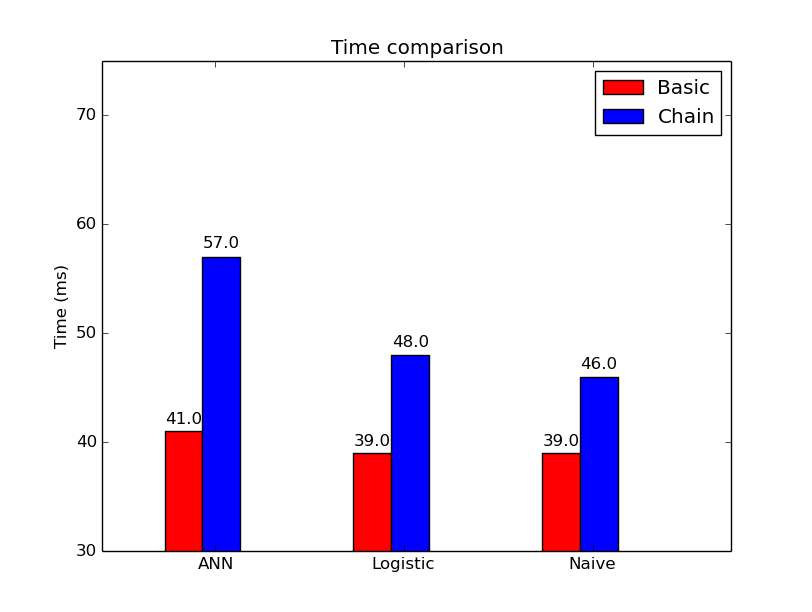
\includegraphics[scale=0.6]{figures/time1_tot.png}
	\end{center}
	
	\caption{Time spent only on processor.}
	\label{pic:time1_tot}

\end{figure}

Naive Bayes' training also has an $O(n)$ complexity for $n$ features. For the other two algorithms, as we saw before, training is done iteratively, until the solutions converge, or a maximum number of iterations is reached. For these reasons, in order to analyse the performance, we monitored the execution time.

Fig. \ref{pic:time1_tot} details the actual computation time or the time the program spent on the processor doing just mathematical operations, while Fig. \ref{pic:time2_tot} details a full execution including the time spent preparing the data. 

One test case for an algorithm represents a loop with 30 iterations. In each iteration, the algorithm is trained once. For every algorithm, 1000 test cases have been executed and the results averaged, obtaining the numbers appearing in Fig. \ref{pic:time1_tot} and Fig. \ref{pic:time2_tot}. The measurements have been done with the \textit{time} command available on most UNIX/LINUX systems. 

\begin{figure}[h]
	\begin{center}
		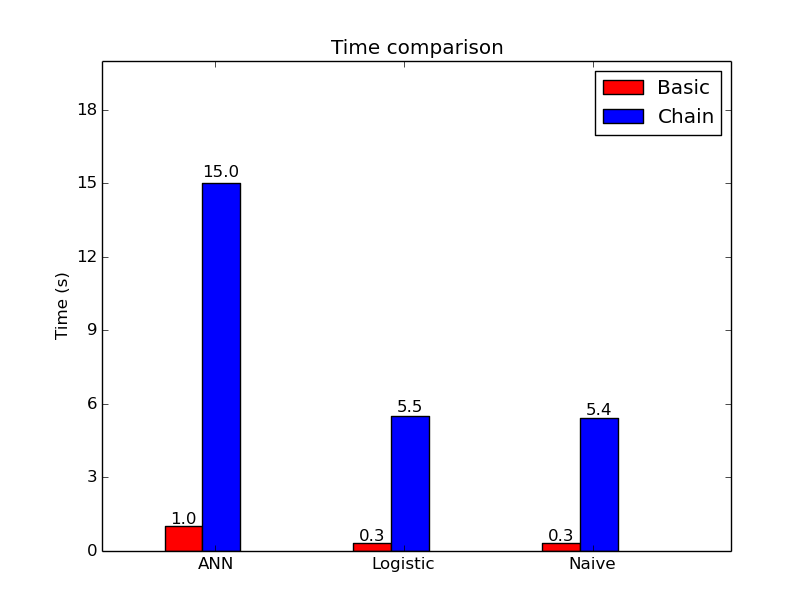
\includegraphics[scale=0.6]{figures/time2_tot.png}
	\end{center}
	
	\caption{Full execution time for algorithms.}
	\label{pic:time2_tot}

\end{figure}

Let us first discuss the time spent only on the processor. When using only measured Bluetooth RSSI, the results are very similar, with only a slight increase for ANN. This can be explained by simple form the classifiers take when using only one feature. Obviously, when we use two features, we will observe a time increase across the board. What is interesting is that the ANN execution time increases significantly compared to the other two. Again, this is not unexpected, as the theory behind the algorithms has shown that ANN is the more complex one. Another reason for the time increase is the increase in the number of \textit{neurons} in the hidden layer. This is required in order to obtain the same accuracy as the other two algorithms.

The full execution time for the algorithms tells a similar story. The same trend applies, where the logistic regression and Naive Bayes are faster than the neural network. However differences are more pronounced. For the base case, while before, the ANN was only slightly slower than the other two, now it is almost 3 times as slow. The structures needed to be created and allocated in order to hold an ANN in memory play a big part in this difference, even if just one feature is used. 

Also, the time difference between the base case and the one using chain length is significantly more higher. While the increase in the number of features certainly has an effect on this difference, it is eclipsed by the data processing part. Extracting just the RSSI of a known time window is a relatively cheap task, while parsing an entire chain to determine its length comes with an extremely high cost. 

From a complexity point of view, we have a clear result. Both logistic regression and Naive Bayes have similar results, with both being better than the ANN. 
                                     %Chapter 3
\appendix
\chapter{Appendix}

\section{Examples of data formats from SensibleDTU app}

The data displayed here is not real, but the format is accurate. 

\begin{lstlisting}
{"timestamp_added": 1326129999, "name": "edu.mit.media.funf.probe.builtin.BluetoothProbe", "timestamp": 1384118284, "probe": "edu_mit_media_funf_probe_builtin_BluetoothProbe", "uuid": "1b3f4fe8-fffb-445c-bf52-5277ba67159-v0.3.2.4-0.5", "user": "d82fd5ca764f93bc38de04987ff13f", "device": "97e4ac7b-5aad-4190-83ac-b1f5ab40e487", "device_bt_mac": "E4:B0:21:E2:BF:10", "_id": "b21f904210a5a2b2cf408fa1cd2e34db_d82fa764f93bc3887ff13f_138297", "data": {"TIMESTAMP": 1394118297, "PROBE": "edu.mit.media.funf.probe.builtin.BluetoothProbe", "DEVICES": [{"android_bluetooth_device_extra_DEVICE": {"mAddress": "6e96626852eeaa41a2922780aff31767c6e842f34b20acffa49f6cb03"}, "android_bluetooth_device_extra_CLASS": {"mClass": 1573132}, "android_bluetooth_device_extra_RSSI": -73, "android_bluetooth_device_extra_NAME": "278450befb3d42372af5556577d0d9d"}, {"android_bluetooth_device_extra_DEVICE": {"mAddress": "f0ce0583a6c2f6743ccd8ed3a6f27b14c280c0c0cc4b1ed478"}, "android_bluetooth_device_extra_CLASS": {"mClass": 3801356}, "android_bluetooth_device_extra_RSSI": -78, "android_bluetooth_device_extra_NAME": "3db16e2f261af1c8c88ae88b0a9d546e2ab3e7329179"}]}, "sensible_token": "8e1754d8090059f8c4910d8897", "device_id": "bd955a5204e7e08de0eae2d9002d77e2"}
\end{lstlisting}

\begin{lstlisting}
"1b768078564005168dda562defa5b","1d7786b4b125656f74","ce4ad2c34123553c3b72b60e4eab19971456f5f391ed7","-82","2014-03-19 10:57:43"
"1b768f942564005168dda562defa5b","1d7786b4b121679bb9b5800eb46f74","9835c86c172aa3398564112455b42f54009a1ce37478d905f998d3f6c7","-73","2014-03-19 10:57:43"
"1b768f9412450516332defa5b","1d7786b4b13d04679bb9b58643b46f74","818dd0f1afd862c52b112262709c641b1995567ba28c3c20e","-57","2014-03-19 10:57:43"
"1b768f942564005168dda562defa5b","1d778234b13d04679bb9b5800eb46f74","8547c45679a561f8cbfff70de8572f161206ea06ce380a973","-88","2014-03-19 10:57:43"
"1b768f9425641234dda562defa5b","1d7786b412379bb9b5800eb46f74","818dd0f1afd862c52b8bdd65c37562709c641b19977c4ba1315057ba28c3c20e","-55","2014-03-19 11:02:43"
"1b768f942564005168444efa5b","1d7786b412323679bb9b5800eb46f74","ce4ad2c3477aef48ca1431004c023c3b72b60e4eab199712391ed7","-90","2014-03-19 11:02:43"
\end{lstlisting}


\section{The SensibleDTU data collection app}

Fig~\ref{pic:sensapp} shows the SensibleDTU data collection app login screen. 

\begin{figure}[h]
	\begin{center}
		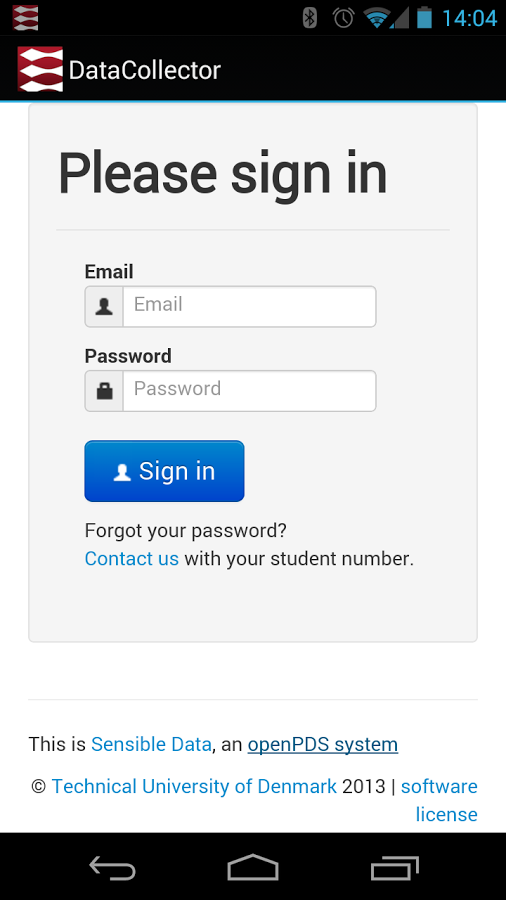
\includegraphics[scale=0.4]{figures/sensibleapp.png}
	\end{center}
	
	\caption{SensibleDTU data collection app.}
	\label{pic:sensapp}

\end{figure}                                 %Appendix A
%-----------
% Backmatter
%-----------
\backmatter
\chaptermark{Bibliography}
\renewcommand{\sectionmark}[1]{\markright{#1}}
\sectionmark{Bibliography}
\addcontentsline{toc}{chapter}{Bibliography}        %Force addition of Bibliography to TOC
\bibliographystyle{alpha}                           %Use alpha codes for references
\bibliography{References}                           %Bibliography file called
\end{document}
% % % EOF % % %